\documentclass[a4paper, 14pt]{article}
\usepackage[T2A]{fontenc}
\usepackage[utf8]{inputenc}
\usepackage[english,russian]{babel}
\usepackage[top = 2cm, bottom = 2 cm]{geometry}
\usepackage{cmap}
\usepackage{graphicx}
\usepackage{listings}
\usepackage{color}
\usepackage{amsmath}
\usepackage{pgfplots}
\usepackage{url}
\usepackage{tikz}
\usepackage{float}
\usepackage{multirow}
\usepackage{pdfpages}

\usepackage{titlesec}
\titleformat*{\section}{\LARGE\bfseries}
\titleformat*{\subsection}{\Large\bfseries}
\titleformat*{\subsubsection}{\large\bfseries}
\titleformat*{\paragraph}{\large\bfseries}
\titleformat*{\subparagraph}{\large\bfseries}


\begin{document}


\includepdf[pages={1}]{title.pdf}

\textbf{Цель работы:} реализовать программу для построения графиков функции и плотности следующих распределений:
\begin{enumerate}
    \item равномерное распределение;
    \item экспоненциальное распределение. 
\end{enumerate}
	
\section*{Равномерное распределение}
	
Равномерное распределение - распределение случайной величины, принимающей значения, принадлежащие некоторому промежутку конечной длины, характеризующееся тем, что плотность вероятности на этом промежутке всюду постоянна.\\

Функция распределения:

\begin{equation*}
F_X (x) =
    \begin{cases}
        0, & x < a \\
        \frac{x - a}{b - a}, & a \le x < b \\
        1, & x \geq b \\
    \end{cases}
\end{equation*}
	
Плотность распределения:

\begin{equation*}
    f_X (x) =
    \begin{cases}
        \frac{1}{b-a}, & x \in [a,b] \\
        0, & x \notin [a, b] \\
    \end{cases}
\end{equation*}


\section*{Экспоненциальное распределение}

Функция распределения:

\begin{equation*}
F_X (x) =
    \begin{cases}
        1 - e^{-\lambda x},& x \geq 0 \\
        0, & x < 0 \\
    \end{cases}
\end{equation*}
	
Плотность распределения:

\begin{equation*}
    f_X (x) =
    \begin{cases}
        \lambda e^{-\lambda x},& x \geq 0 \\
        0, & x < 0 \\
    \end{cases}
\end{equation*}

\section*{Результаты работы}

В результате работы были полученые следующие графики распределения и плотности распределения

\begin{figure}[H]
    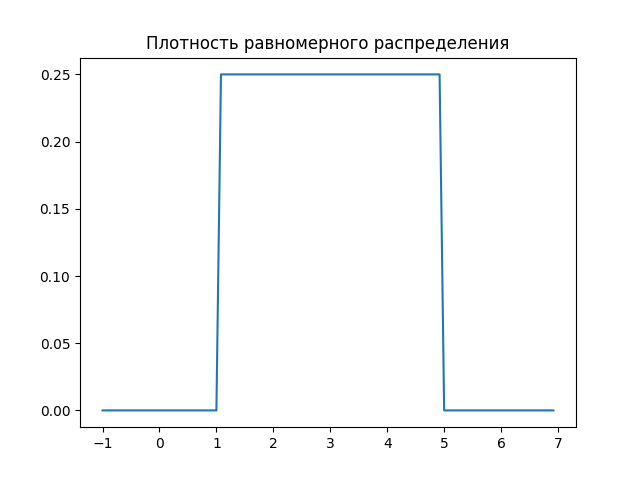
\includegraphics[scale=0.8]{1_5_uniform_density.png}
    \caption{Плотность равномерного распределения при $a = 1, b = 5$}
\end{figure}

\begin{figure}[H]
    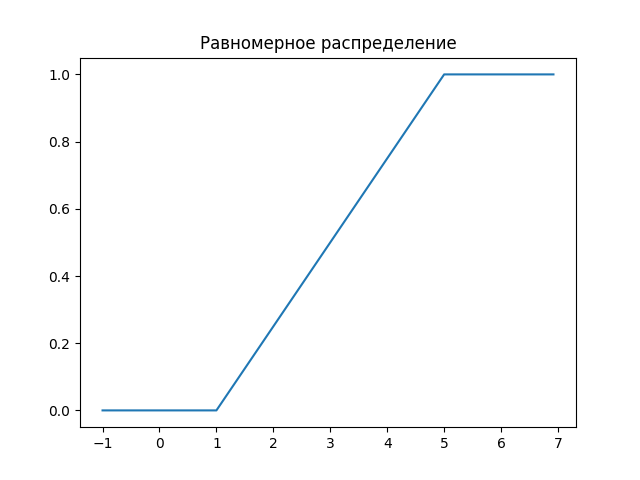
\includegraphics[scale=0.8]{1_5_uniform.png}
    \caption{Равномерное распределение при $a = 1, b = 5$}
\end{figure}

\begin{figure}[H]
    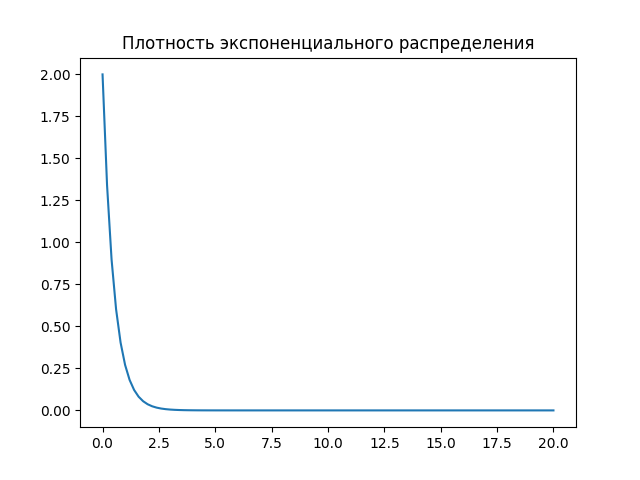
\includegraphics[scale=0.8]{2_exponential_density.png}
    \caption{Экспоненциальное распределение при $\lambda=2$}
\end{figure}

\begin{figure}[H]
    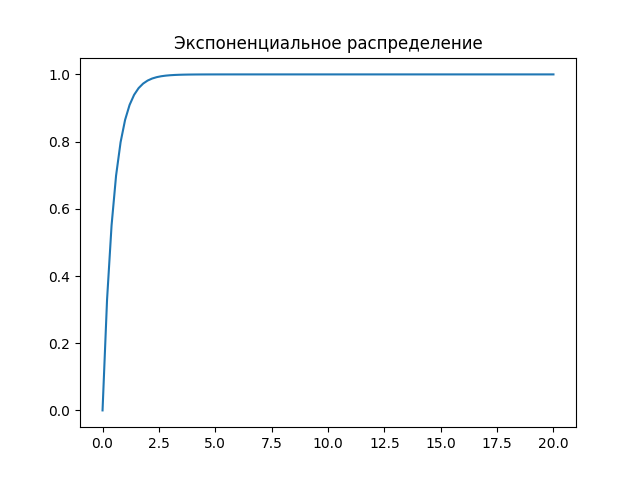
\includegraphics[scale=0.8]{2_exponential.png}
    \caption{Экспоненциальное распределение при $\lambda=0.2$}
\end{figure}

\begin{figure}[H]
    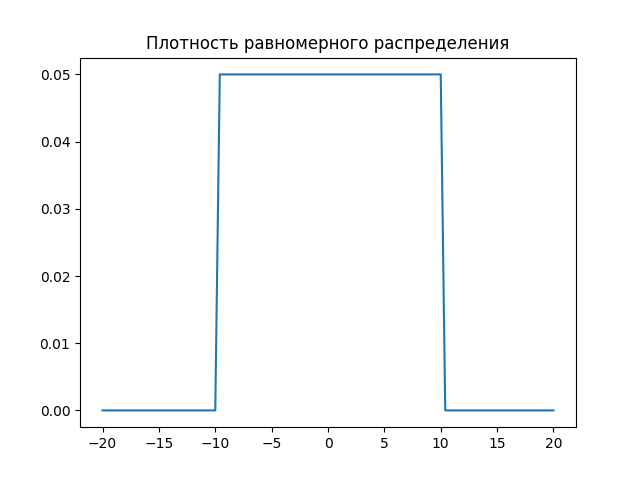
\includegraphics[scale=0.8]{-10_10_uniform_density.png}
    \caption{Плотность равномерного распределения при $a = -10, b = 10$}
\end{figure}

\begin{figure}[H]
    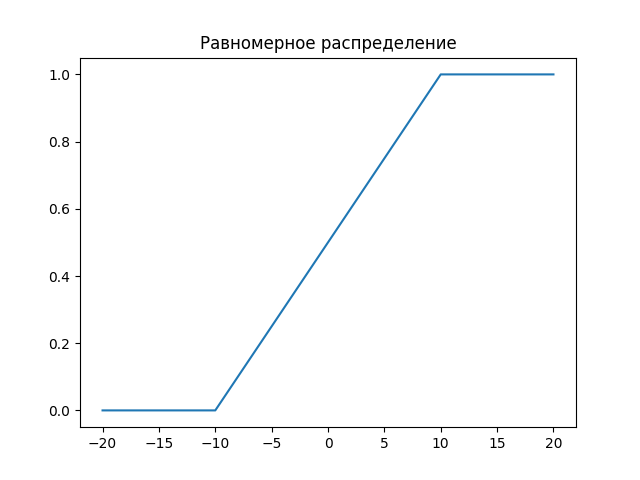
\includegraphics[scale=0.8]{-10_10_uniform.png}
    \caption{Равномерное распределение при $a = -10, b = 10$}
\end{figure}

\begin{figure}[H]
    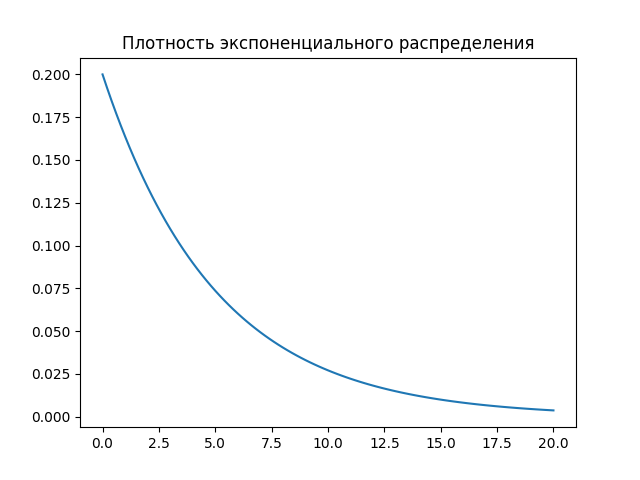
\includegraphics[scale=0.8]{02_exponential_density.png}
    \caption{Плотность экспоненциального распределения при $\lambda=0.2$}
\end{figure}

\begin{figure}[H]
    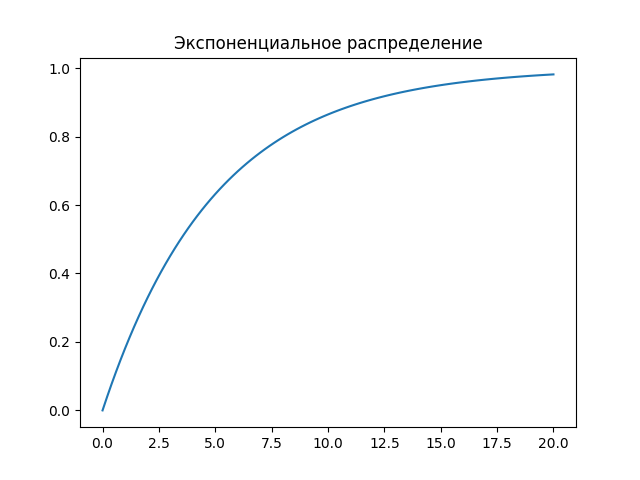
\includegraphics[scale=0.8]{02_exponential.png}
    \caption{Экспоненциальное распределение при $\lambda=0.2$}
\end{figure}

\section*{Вывод}
В ходе выполнения лабораторной работы была реализована программа для построения графиков функции и плотности равномерного распределения и экспоненциального распределения. Были построены графики при различных параметрах $a, b$ для равномерного распределения и $\lambda$ для экспоненциального распределения и их плотностей.
\end{document}